% Created by tikzDevice version 0.12.3.1 on 2021-07-02 12:57:41
% !TEX encoding = UTF-8 Unicode
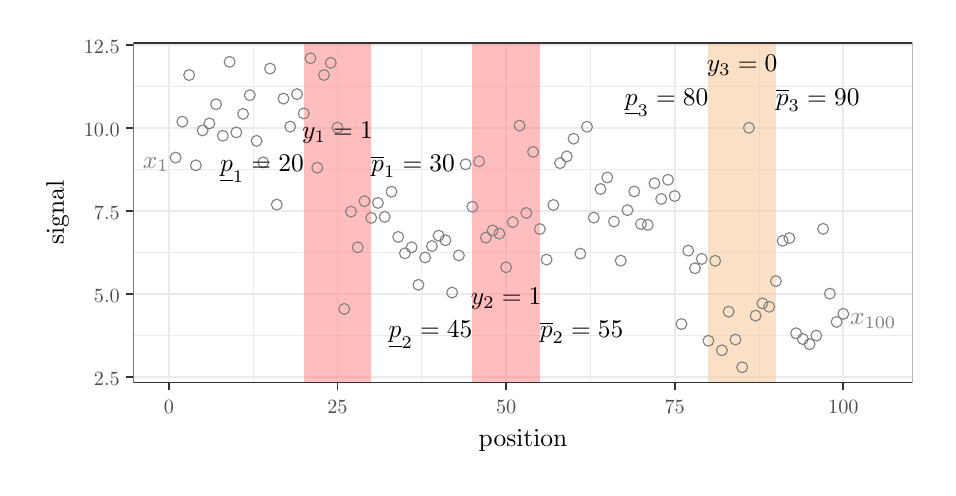
\begin{tikzpicture}[x=1pt,y=1pt]
\definecolor{fillColor}{RGB}{255,255,255}
\path[use as bounding box,fill=fillColor,fill opacity=0.00] (0,0) rectangle (325.21,158.99);
\begin{scope}
\path[clip] (  0.00,  0.00) rectangle (325.21,158.99);
\definecolor{drawColor}{RGB}{255,255,255}
\definecolor{fillColor}{RGB}{255,255,255}

\path[draw=drawColor,line width= 0.6pt,line join=round,line cap=round,fill=fillColor] (  0.00,  0.00) rectangle (325.21,158.99);
\end{scope}
\begin{scope}
\path[clip] ( 38.23, 30.69) rectangle (319.71,153.49);
\definecolor{fillColor}{RGB}{255,255,255}

\path[fill=fillColor] ( 38.23, 30.69) rectangle (319.71,153.49);
\definecolor{drawColor}{gray}{0.92}

\path[draw=drawColor,line width= 0.3pt,line join=round] ( 38.23, 47.77) --
	(319.71, 47.77);

\path[draw=drawColor,line width= 0.3pt,line join=round] ( 38.23, 77.78) --
	(319.71, 77.78);

\path[draw=drawColor,line width= 0.3pt,line join=round] ( 38.23,107.80) --
	(319.71,107.80);

\path[draw=drawColor,line width= 0.3pt,line join=round] ( 38.23,137.82) --
	(319.71,137.82);

\path[draw=drawColor,line width= 0.3pt,line join=round] ( 81.49, 30.69) --
	( 81.49,153.49);

\path[draw=drawColor,line width= 0.3pt,line join=round] (142.42, 30.69) --
	(142.42,153.49);

\path[draw=drawColor,line width= 0.3pt,line join=round] (203.34, 30.69) --
	(203.34,153.49);

\path[draw=drawColor,line width= 0.3pt,line join=round] (264.27, 30.69) --
	(264.27,153.49);

\path[draw=drawColor,line width= 0.6pt,line join=round] ( 38.23, 32.76) --
	(319.71, 32.76);

\path[draw=drawColor,line width= 0.6pt,line join=round] ( 38.23, 62.78) --
	(319.71, 62.78);

\path[draw=drawColor,line width= 0.6pt,line join=round] ( 38.23, 92.79) --
	(319.71, 92.79);

\path[draw=drawColor,line width= 0.6pt,line join=round] ( 38.23,122.81) --
	(319.71,122.81);

\path[draw=drawColor,line width= 0.6pt,line join=round] ( 38.23,152.82) --
	(319.71,152.82);

\path[draw=drawColor,line width= 0.6pt,line join=round] ( 51.02, 30.69) --
	( 51.02,153.49);

\path[draw=drawColor,line width= 0.6pt,line join=round] (111.95, 30.69) --
	(111.95,153.49);

\path[draw=drawColor,line width= 0.6pt,line join=round] (172.88, 30.69) --
	(172.88,153.49);

\path[draw=drawColor,line width= 0.6pt,line join=round] (233.81, 30.69) --
	(233.81,153.49);

\path[draw=drawColor,line width= 0.6pt,line join=round] (294.73, 30.69) --
	(294.73,153.49);
\definecolor{drawColor}{gray}{0.50}

\node[text=drawColor,anchor=base east,inner sep=0pt, outer sep=0pt, scale=  0.92] at ( 51.02,108.24) {$x_{1}$};

\node[text=drawColor,anchor=base west,inner sep=0pt, outer sep=0pt, scale=  0.92] at (297.17, 51.76) {$x_{100}$};
\definecolor{fillColor}{RGB}{255,125,125}

\path[fill=fillColor,fill opacity=0.50] ( 99.77, 30.69) rectangle (124.14,153.49);

\path[fill=fillColor,fill opacity=0.50] (160.69, 30.69) rectangle (185.06,153.49);
\definecolor{fillColor}{RGB}{246,196,143}

\path[fill=fillColor,fill opacity=0.50] (245.99, 30.69) rectangle (270.36,153.49);

\path[draw=drawColor,line width= 0.4pt,line join=round,line cap=round] ( 53.46,112.04) circle (  1.96);

\path[draw=drawColor,line width= 0.4pt,line join=round,line cap=round] ( 55.90,125.03) circle (  1.96);

\path[draw=drawColor,line width= 0.4pt,line join=round,line cap=round] ( 58.34,141.87) circle (  1.96);

\path[draw=drawColor,line width= 0.4pt,line join=round,line cap=round] ( 60.77,109.24) circle (  1.96);

\path[draw=drawColor,line width= 0.4pt,line join=round,line cap=round] ( 63.21,121.85) circle (  1.96);

\path[draw=drawColor,line width= 0.4pt,line join=round,line cap=round] ( 65.65,124.40) circle (  1.96);

\path[draw=drawColor,line width= 0.4pt,line join=round,line cap=round] ( 68.08,131.31) circle (  1.96);

\path[draw=drawColor,line width= 0.4pt,line join=round,line cap=round] ( 70.52,119.93) circle (  1.96);

\path[draw=drawColor,line width= 0.4pt,line join=round,line cap=round] ( 72.96,146.63) circle (  1.96);

\path[draw=drawColor,line width= 0.4pt,line join=round,line cap=round] ( 75.39,121.14) circle (  1.96);

\path[draw=drawColor,line width= 0.4pt,line join=round,line cap=round] ( 77.83,127.82) circle (  1.96);

\path[draw=drawColor,line width= 0.4pt,line join=round,line cap=round] ( 80.27,134.60) circle (  1.96);

\path[draw=drawColor,line width= 0.4pt,line join=round,line cap=round] ( 82.71,118.09) circle (  1.96);

\path[draw=drawColor,line width= 0.4pt,line join=round,line cap=round] ( 85.14,110.33) circle (  1.96);

\path[draw=drawColor,line width= 0.4pt,line join=round,line cap=round] ( 87.58,144.21) circle (  1.96);

\path[draw=drawColor,line width= 0.4pt,line join=round,line cap=round] ( 90.02, 95.06) circle (  1.96);

\path[draw=drawColor,line width= 0.4pt,line join=round,line cap=round] ( 92.45,133.36) circle (  1.96);

\path[draw=drawColor,line width= 0.4pt,line join=round,line cap=round] ( 94.89,123.24) circle (  1.96);

\path[draw=drawColor,line width= 0.4pt,line join=round,line cap=round] ( 97.33,134.97) circle (  1.96);

\path[draw=drawColor,line width= 0.4pt,line join=round,line cap=round] ( 99.77,128.00) circle (  1.96);

\path[draw=drawColor,line width= 0.4pt,line join=round,line cap=round] (102.20,147.91) circle (  1.96);

\path[draw=drawColor,line width= 0.4pt,line join=round,line cap=round] (104.64,108.40) circle (  1.96);

\path[draw=drawColor,line width= 0.4pt,line join=round,line cap=round] (107.08,141.89) circle (  1.96);

\path[draw=drawColor,line width= 0.4pt,line join=round,line cap=round] (109.51,146.28) circle (  1.96);

\path[draw=drawColor,line width= 0.4pt,line join=round,line cap=round] (111.95,122.87) circle (  1.96);

\path[draw=drawColor,line width= 0.4pt,line join=round,line cap=round] (114.39, 57.35) circle (  1.96);

\path[draw=drawColor,line width= 0.4pt,line join=round,line cap=round] (116.83, 92.52) circle (  1.96);

\path[draw=drawColor,line width= 0.4pt,line join=round,line cap=round] (119.26, 79.63) circle (  1.96);

\path[draw=drawColor,line width= 0.4pt,line join=round,line cap=round] (121.70, 96.30) circle (  1.96);

\path[draw=drawColor,line width= 0.4pt,line join=round,line cap=round] (124.14, 90.27) circle (  1.96);

\path[draw=drawColor,line width= 0.4pt,line join=round,line cap=round] (126.57, 95.66) circle (  1.96);

\path[draw=drawColor,line width= 0.4pt,line join=round,line cap=round] (129.01, 90.62) circle (  1.96);

\path[draw=drawColor,line width= 0.4pt,line join=round,line cap=round] (131.45, 99.71) circle (  1.96);

\path[draw=drawColor,line width= 0.4pt,line join=round,line cap=round] (133.89, 83.38) circle (  1.96);

\path[draw=drawColor,line width= 0.4pt,line join=round,line cap=round] (136.32, 77.46) circle (  1.96);

\path[draw=drawColor,line width= 0.4pt,line join=round,line cap=round] (138.76, 79.64) circle (  1.96);

\path[draw=drawColor,line width= 0.4pt,line join=round,line cap=round] (141.20, 66.07) circle (  1.96);

\path[draw=drawColor,line width= 0.4pt,line join=round,line cap=round] (143.63, 75.95) circle (  1.96);

\path[draw=drawColor,line width= 0.4pt,line join=round,line cap=round] (146.07, 80.08) circle (  1.96);

\path[draw=drawColor,line width= 0.4pt,line join=round,line cap=round] (148.51, 83.83) circle (  1.96);

\path[draw=drawColor,line width= 0.4pt,line join=round,line cap=round] (150.95, 82.18) circle (  1.96);

\path[draw=drawColor,line width= 0.4pt,line join=round,line cap=round] (153.38, 63.27) circle (  1.96);

\path[draw=drawColor,line width= 0.4pt,line join=round,line cap=round] (155.82, 76.68) circle (  1.96);

\path[draw=drawColor,line width= 0.4pt,line join=round,line cap=round] (158.26,109.64) circle (  1.96);

\path[draw=drawColor,line width= 0.4pt,line join=round,line cap=round] (160.69, 94.26) circle (  1.96);

\path[draw=drawColor,line width= 0.4pt,line join=round,line cap=round] (163.13,110.69) circle (  1.96);

\path[draw=drawColor,line width= 0.4pt,line join=round,line cap=round] (165.57, 83.12) circle (  1.96);

\path[draw=drawColor,line width= 0.4pt,line join=round,line cap=round] (168.00, 85.70) circle (  1.96);

\path[draw=drawColor,line width= 0.4pt,line join=round,line cap=round] (170.44, 84.58) circle (  1.96);

\path[draw=drawColor,line width= 0.4pt,line join=round,line cap=round] (172.88, 72.40) circle (  1.96);

\path[draw=drawColor,line width= 0.4pt,line join=round,line cap=round] (175.32, 88.73) circle (  1.96);

\path[draw=drawColor,line width= 0.4pt,line join=round,line cap=round] (177.75,123.60) circle (  1.96);

\path[draw=drawColor,line width= 0.4pt,line join=round,line cap=round] (180.19, 92.05) circle (  1.96);

\path[draw=drawColor,line width= 0.4pt,line join=round,line cap=round] (182.63,114.11) circle (  1.96);

\path[draw=drawColor,line width= 0.4pt,line join=round,line cap=round] (185.06, 86.22) circle (  1.96);

\path[draw=drawColor,line width= 0.4pt,line join=round,line cap=round] (187.50, 75.19) circle (  1.96);

\path[draw=drawColor,line width= 0.4pt,line join=round,line cap=round] (189.94, 94.92) circle (  1.96);

\path[draw=drawColor,line width= 0.4pt,line join=round,line cap=round] (192.38,110.03) circle (  1.96);

\path[draw=drawColor,line width= 0.4pt,line join=round,line cap=round] (194.81,112.47) circle (  1.96);

\path[draw=drawColor,line width= 0.4pt,line join=round,line cap=round] (197.25,118.87) circle (  1.96);

\path[draw=drawColor,line width= 0.4pt,line join=round,line cap=round] (199.69, 77.33) circle (  1.96);

\path[draw=drawColor,line width= 0.4pt,line join=round,line cap=round] (202.12,123.18) circle (  1.96);

\path[draw=drawColor,line width= 0.4pt,line join=round,line cap=round] (204.56, 90.35) circle (  1.96);

\path[draw=drawColor,line width= 0.4pt,line join=round,line cap=round] (207.00,100.70) circle (  1.96);

\path[draw=drawColor,line width= 0.4pt,line join=round,line cap=round] (209.44,104.87) circle (  1.96);

\path[draw=drawColor,line width= 0.4pt,line join=round,line cap=round] (211.87, 88.95) circle (  1.96);

\path[draw=drawColor,line width= 0.4pt,line join=round,line cap=round] (214.31, 74.80) circle (  1.96);

\path[draw=drawColor,line width= 0.4pt,line join=round,line cap=round] (216.75, 93.04) circle (  1.96);

\path[draw=drawColor,line width= 0.4pt,line join=round,line cap=round] (219.18, 99.81) circle (  1.96);

\path[draw=drawColor,line width= 0.4pt,line join=round,line cap=round] (221.62, 88.04) circle (  1.96);

\path[draw=drawColor,line width= 0.4pt,line join=round,line cap=round] (224.06, 87.73) circle (  1.96);

\path[draw=drawColor,line width= 0.4pt,line join=round,line cap=round] (226.50,102.76) circle (  1.96);

\path[draw=drawColor,line width= 0.4pt,line join=round,line cap=round] (228.93, 97.10) circle (  1.96);

\path[draw=drawColor,line width= 0.4pt,line join=round,line cap=round] (231.37,104.02) circle (  1.96);

\path[draw=drawColor,line width= 0.4pt,line join=round,line cap=round] (233.81, 98.15) circle (  1.96);

\path[draw=drawColor,line width= 0.4pt,line join=round,line cap=round] (236.24, 51.89) circle (  1.96);

\path[draw=drawColor,line width= 0.4pt,line join=round,line cap=round] (238.68, 78.43) circle (  1.96);

\path[draw=drawColor,line width= 0.4pt,line join=round,line cap=round] (241.12, 72.04) circle (  1.96);

\path[draw=drawColor,line width= 0.4pt,line join=round,line cap=round] (243.56, 75.41) circle (  1.96);

\path[draw=drawColor,line width= 0.4pt,line join=round,line cap=round] (245.99, 45.85) circle (  1.96);

\path[draw=drawColor,line width= 0.4pt,line join=round,line cap=round] (248.43, 74.74) circle (  1.96);

\path[draw=drawColor,line width= 0.4pt,line join=round,line cap=round] (250.87, 42.42) circle (  1.96);

\path[draw=drawColor,line width= 0.4pt,line join=round,line cap=round] (253.30, 56.37) circle (  1.96);

\path[draw=drawColor,line width= 0.4pt,line join=round,line cap=round] (255.74, 46.30) circle (  1.96);

\path[draw=drawColor,line width= 0.4pt,line join=round,line cap=round] (258.18, 36.27) circle (  1.96);

\path[draw=drawColor,line width= 0.4pt,line join=round,line cap=round] (260.62,122.81) circle (  1.96);

\path[draw=drawColor,line width= 0.4pt,line join=round,line cap=round] (263.05, 54.93) circle (  1.96);

\path[draw=drawColor,line width= 0.4pt,line join=round,line cap=round] (265.49, 59.36) circle (  1.96);

\path[draw=drawColor,line width= 0.4pt,line join=round,line cap=round] (267.93, 58.13) circle (  1.96);

\path[draw=drawColor,line width= 0.4pt,line join=round,line cap=round] (270.36, 67.42) circle (  1.96);

\path[draw=drawColor,line width= 0.4pt,line join=round,line cap=round] (272.80, 81.99) circle (  1.96);

\path[draw=drawColor,line width= 0.4pt,line join=round,line cap=round] (275.24, 82.96) circle (  1.96);

\path[draw=drawColor,line width= 0.4pt,line join=round,line cap=round] (277.67, 48.57) circle (  1.96);

\path[draw=drawColor,line width= 0.4pt,line join=round,line cap=round] (280.11, 46.47) circle (  1.96);

\path[draw=drawColor,line width= 0.4pt,line join=round,line cap=round] (282.55, 44.62) circle (  1.96);

\path[draw=drawColor,line width= 0.4pt,line join=round,line cap=round] (284.99, 47.73) circle (  1.96);

\path[draw=drawColor,line width= 0.4pt,line join=round,line cap=round] (287.42, 86.30) circle (  1.96);

\path[draw=drawColor,line width= 0.4pt,line join=round,line cap=round] (289.86, 62.87) circle (  1.96);

\path[draw=drawColor,line width= 0.4pt,line join=round,line cap=round] (292.30, 52.66) circle (  1.96);

\path[draw=drawColor,line width= 0.4pt,line join=round,line cap=round] (294.73, 55.56) circle (  1.96);
\definecolor{drawColor}{RGB}{0,0,0}

\node[text=drawColor,anchor=base east,inner sep=0pt, outer sep=0pt, scale=  0.92] at ( 99.77,107.00) {$\underline p_{1}=20$};

\node[text=drawColor,anchor=base east,inner sep=0pt, outer sep=0pt, scale=  0.92] at (160.69, 46.97) {$\underline p_{2}=45$};

\node[text=drawColor,anchor=base east,inner sep=0pt, outer sep=0pt, scale=  0.92] at (245.99,131.01) {$\underline p_{3}=80$};

\node[text=drawColor,anchor=base,inner sep=0pt, outer sep=0pt, scale=  0.92] at (111.95,119.01) {$y_{1}=1$};

\node[text=drawColor,anchor=base,inner sep=0pt, outer sep=0pt, scale=  0.92] at (172.88, 58.98) {$y_{2}=1$};

\node[text=drawColor,anchor=base,inner sep=0pt, outer sep=0pt, scale=  0.92] at (258.18,143.02) {$y_{3}=0$};

\node[text=drawColor,anchor=base west,inner sep=0pt, outer sep=0pt, scale=  0.92] at (124.14,107.00) {$\overline p_{1}=30$};

\node[text=drawColor,anchor=base west,inner sep=0pt, outer sep=0pt, scale=  0.92] at (185.06, 46.97) {$\overline p_{2}=55$};

\node[text=drawColor,anchor=base west,inner sep=0pt, outer sep=0pt, scale=  0.92] at (270.36,131.01) {$\overline p_{3}=90$};
\definecolor{drawColor}{gray}{0.20}

\path[draw=drawColor,line width= 0.6pt,line join=round,line cap=round] ( 38.23, 30.69) rectangle (319.71,153.49);
\end{scope}
\begin{scope}
\path[clip] (  0.00,  0.00) rectangle (325.21,158.99);
\definecolor{drawColor}{gray}{0.30}

\node[text=drawColor,anchor=base east,inner sep=0pt, outer sep=0pt, scale=  0.73] at ( 33.28, 29.73) {2.5};

\node[text=drawColor,anchor=base east,inner sep=0pt, outer sep=0pt, scale=  0.73] at ( 33.28, 59.75) {5.0};

\node[text=drawColor,anchor=base east,inner sep=0pt, outer sep=0pt, scale=  0.73] at ( 33.28, 89.76) {7.5};

\node[text=drawColor,anchor=base east,inner sep=0pt, outer sep=0pt, scale=  0.73] at ( 33.28,119.78) {10.0};

\node[text=drawColor,anchor=base east,inner sep=0pt, outer sep=0pt, scale=  0.73] at ( 33.28,149.79) {12.5};
\end{scope}
\begin{scope}
\path[clip] (  0.00,  0.00) rectangle (325.21,158.99);
\definecolor{drawColor}{gray}{0.20}

\path[draw=drawColor,line width= 0.6pt,line join=round] ( 35.48, 32.76) --
	( 38.23, 32.76);

\path[draw=drawColor,line width= 0.6pt,line join=round] ( 35.48, 62.78) --
	( 38.23, 62.78);

\path[draw=drawColor,line width= 0.6pt,line join=round] ( 35.48, 92.79) --
	( 38.23, 92.79);

\path[draw=drawColor,line width= 0.6pt,line join=round] ( 35.48,122.81) --
	( 38.23,122.81);

\path[draw=drawColor,line width= 0.6pt,line join=round] ( 35.48,152.82) --
	( 38.23,152.82);
\end{scope}
\begin{scope}
\path[clip] (  0.00,  0.00) rectangle (325.21,158.99);
\definecolor{drawColor}{gray}{0.20}

\path[draw=drawColor,line width= 0.6pt,line join=round] ( 51.02, 27.94) --
	( 51.02, 30.69);

\path[draw=drawColor,line width= 0.6pt,line join=round] (111.95, 27.94) --
	(111.95, 30.69);

\path[draw=drawColor,line width= 0.6pt,line join=round] (172.88, 27.94) --
	(172.88, 30.69);

\path[draw=drawColor,line width= 0.6pt,line join=round] (233.81, 27.94) --
	(233.81, 30.69);

\path[draw=drawColor,line width= 0.6pt,line join=round] (294.73, 27.94) --
	(294.73, 30.69);
\end{scope}
\begin{scope}
\path[clip] (  0.00,  0.00) rectangle (325.21,158.99);
\definecolor{drawColor}{gray}{0.30}

\node[text=drawColor,anchor=base,inner sep=0pt, outer sep=0pt, scale=  0.73] at ( 51.02, 19.68) {0};

\node[text=drawColor,anchor=base,inner sep=0pt, outer sep=0pt, scale=  0.73] at (111.95, 19.68) {25};

\node[text=drawColor,anchor=base,inner sep=0pt, outer sep=0pt, scale=  0.73] at (172.88, 19.68) {50};

\node[text=drawColor,anchor=base,inner sep=0pt, outer sep=0pt, scale=  0.73] at (233.81, 19.68) {75};

\node[text=drawColor,anchor=base,inner sep=0pt, outer sep=0pt, scale=  0.73] at (294.73, 19.68) {100};
\end{scope}
\begin{scope}
\path[clip] (  0.00,  0.00) rectangle (325.21,158.99);
\definecolor{drawColor}{RGB}{0,0,0}

\node[text=drawColor,anchor=base,inner sep=0pt, outer sep=0pt, scale=  0.92] at (178.97,  7.64) {position};
\end{scope}
\begin{scope}
\path[clip] (  0.00,  0.00) rectangle (325.21,158.99);
\definecolor{drawColor}{RGB}{0,0,0}

\node[text=drawColor,rotate= 90.00,anchor=base,inner sep=0pt, outer sep=0pt, scale=  0.92] at ( 13.08, 92.09) {signal};
\end{scope}
\end{tikzpicture}
